

    \section{POLÍMEROS O MACROMOLÉCULAS. TIPOS}

    Son moléculas muy grandes, con una  masa molecular que puede alcanzar millones de umas, que se obtienen por la
    repetición de una o más unidades simples llamadas “\textbf{monómeros}” unidas entre sí mediante enlaces covalentes.

    Forman largas cadenas que se pueden unirentre sí por fuerzas de Van der Waals o puentes de hidrógeno.

    Se pueden clasificar según diversos criterios:

    \begin{enumerate}[label=\numberballmDarkTeal]
        \item \textbf{Según su origen}.
        \begin{enumerate}[label=\letraminuscula]
            \item \textbf{Naturales}.
            Caucho, polisacáridos (celulosa, almidón),
            proteínas, ácidos nucléicos..
            \item \textbf{Artificiales}. Plásticos,
            fibras textiles sintéticas, poliuretano, baquelita...


        \end{enumerate}
        \item \textbf{Según su composición}.
        \begin{enumerate}[label=\letraminuscula]
            \item \textbf{Homopolímeros}. Un solo monómero.
            \item \textbf{Heteropolímeros}. Varios monómeros. Si son monómeros diferentes se llaman \textbf{copolímeros}.
        \end{enumerate}
        \item \textbf{Según su estructura}.
        \begin{enumerate}[label=\letraminuscula]
            \item \textbf{Lineal}. Los monómeros se unen por dos sitios (cabeza y cola).
            \item \textbf{Ramificados}. Sei algún monómero se puede unir por tres o más sitios.
        \end{enumerate}
        \item \textbf{Por su comportamiento ante el calor}.
        \begin{enumerate}[label=\letraminuscula]
            \item \textbf{Termoplásticos}. Se reblandecen al calentar y recuperan sus propiedades al enfriar. Se moldean en caliente de forma repetida.
            \item \textbf{Termoestables}. Se reblandecen y moldean en caliente, pero quedan rígidos al ser enfriados por formar nuevos enlaces y no pueden volver a ser moldeados.
        \end{enumerate}
    \end{enumerate}


    \section{TIPOS DE POLIMERIZACIÓN}


    Existen dos tipos fundamentales de polimerización:

    \begin{enumerate}[label=\numberballmDarkTeal]
        \item \textbf{Adición}.
        \item \textbf{Condensación}.
    \end{enumerate}

%    \marcador{poner esquema con tipos}
    \begin{figure}[H]
        \centering
        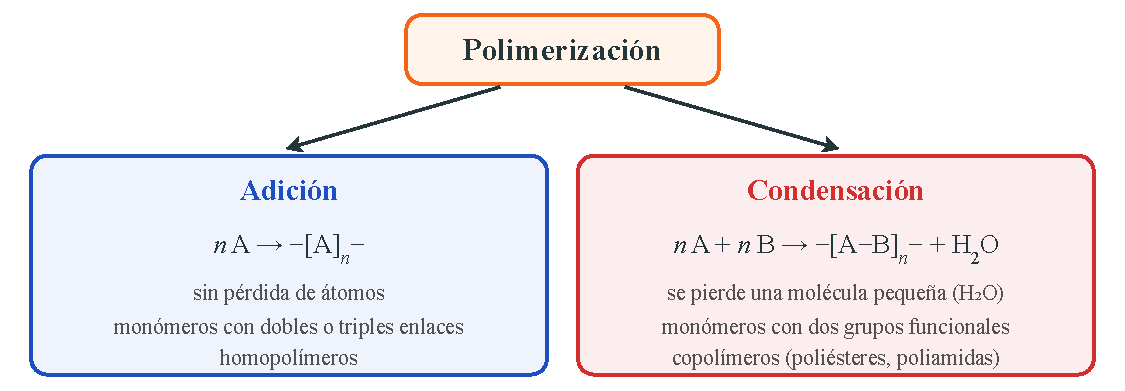
\includegraphics[width=0.85\linewidth]{FigurasSVG/UD10_Polimeros/pdf/UD10_01_tipos_polimerizacion.pdf}
        \caption{Tipos de polimerización}
        \label{fig:tipos-polimerizacion}
    \end{figure}


    \section{Polímeros de adición}

    La masa molecular del polímero es
    un múltiplo exacto de la masa molecular del monómero, pues al formarse la
    cadena los monómeros se unen sin perder ningún átomo. Los monómeros tienen
    insaturaciones (dobles o triples enlaces) que pasan a sencillos en el polímero.


    Suelen seguir un mecanismo en tres fases, con
    ruptura homolítica del enlace:

    \begin{itemize}
        \item \textbf{Iniciación}.% \marcador{poner esquema}
            \begin{figure}[H]
                \centering
                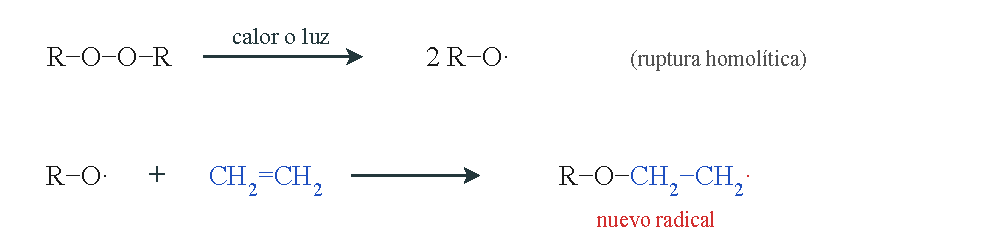
\includegraphics[width=0.8\linewidth]{FigurasSVG/UD10_Polimeros/pdf/UD10_02_iniciacion.pdf}
                \caption{Iniciación de la polimerización por adición}
                \label{fig:polimerizacion-iniciacion}
            \end{figure}
        \item \textbf{Propagación o crecimiento}. % \marcador{poner esquema}
            \begin{figure}[H]
                \centering
                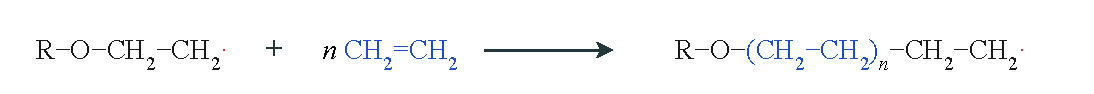
\includegraphics[width=0.9\linewidth]{FigurasSVG/UD10_Polimeros/pdf/UD10_03_propagacion.pdf}
                \caption{Propagación de la cadena}
                \label{fig:polimerizacion-propagacion}
            \end{figure}
        \item \textbf{Terminación}. Los radicales libres de los extremos se unen a impurezas o bien se unen dos cadenas con un terminal neutralizado.
            \begin{figure}[H]
                \centering
                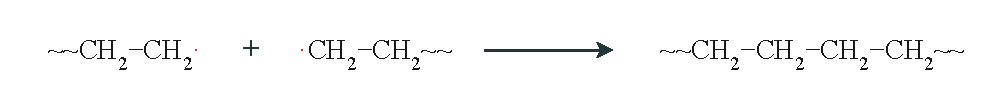
\includegraphics[width=0.8\linewidth]{FigurasSVG/UD10_Polimeros/pdf/UD10_04_terminacion.pdf}
                \caption{Terminación por combinación de dos radicales}
                \label{fig:polimerizacion-terminacion}
            \end{figure}
    \end{itemize}

    Veamos algunos de los polímeros de
    adición más importantes, sus principales aplicaciones, así como los monómeros
    de los que proceden. Nótese que los polímeros de adición son homopolímeros y basan
    su nomenclatura en el nombre comercial de los monómeros.

    \begin{figure}[H]
        \centering
        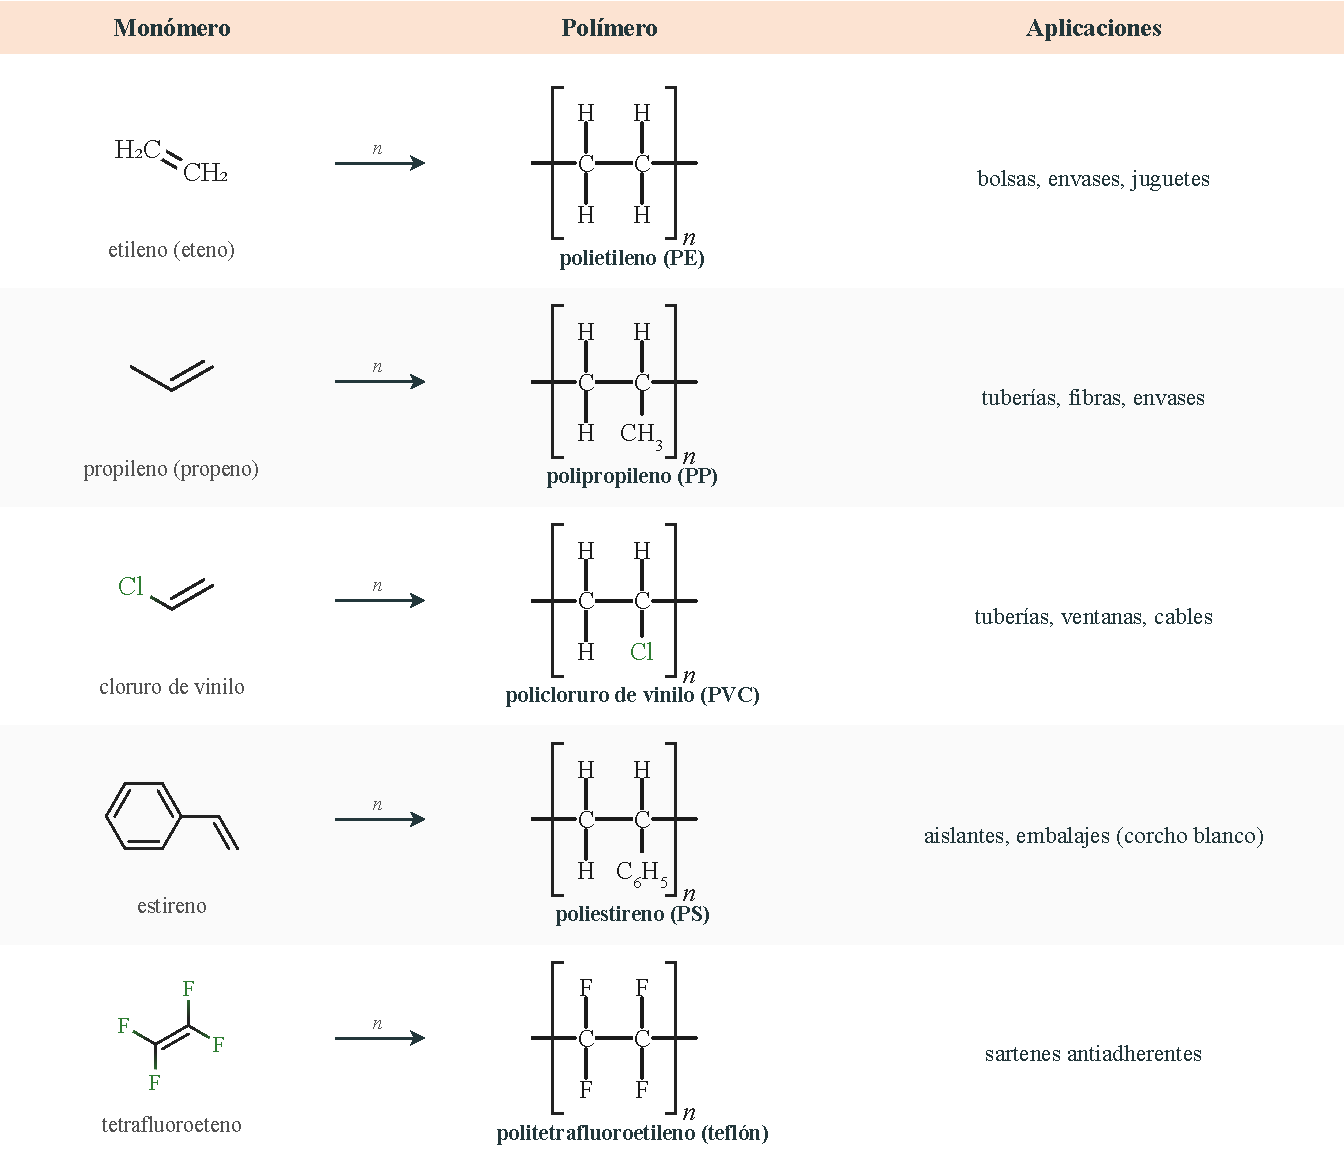
\includegraphics[width=1.0\linewidth]{FigurasSVG/UD10_Polimeros/pdf/UD10_05_polimeros_adicion.pdf}
        \caption{Principales polímeros de adición}
        \label{fig:polimeros-adicion}
    \end{figure}


    \section{Polímeros de condensación}

    Se produce por la unión de monómeros con pérdida de una molécula pequeña, por ejemplo agua. Por tanto, la masa molecular del polímero no es un múltiplo exacto de la masa molecular del monómero. Los polímeros son mucho más pequeños que los de adición y son heteropolímeros (copolímeros), ya que los monómeros de partida tienen que ser distintos.

	Los principales polímeros de condensación son:

    \begin{enumerate}[label=\numberballmDarkTeal]
        \item \negsubro{Poliésteres}. Los poliésteres son unos polímeros que contiene el grupo funcional éster en su cadena principal que se repite \( n \) veces.

        Se producen por sucesivas reacciones de esterificación (alcohol y ácido). Para formar la función éster a los dos lados de la cadena se requiere que uno de los monómeros sea un diácido y el otro un diol terminal.

        El poliéster más conocido es el formado por ácido tereftálico (ácido p-benceno-dicarboxilico) y el etilenglicol (etanodiol) que se puede obtener como fibra textil llamada tergal (dacrón) o como plástico que se conoce como PET:

        \begin{figure}[H]
            \centering
            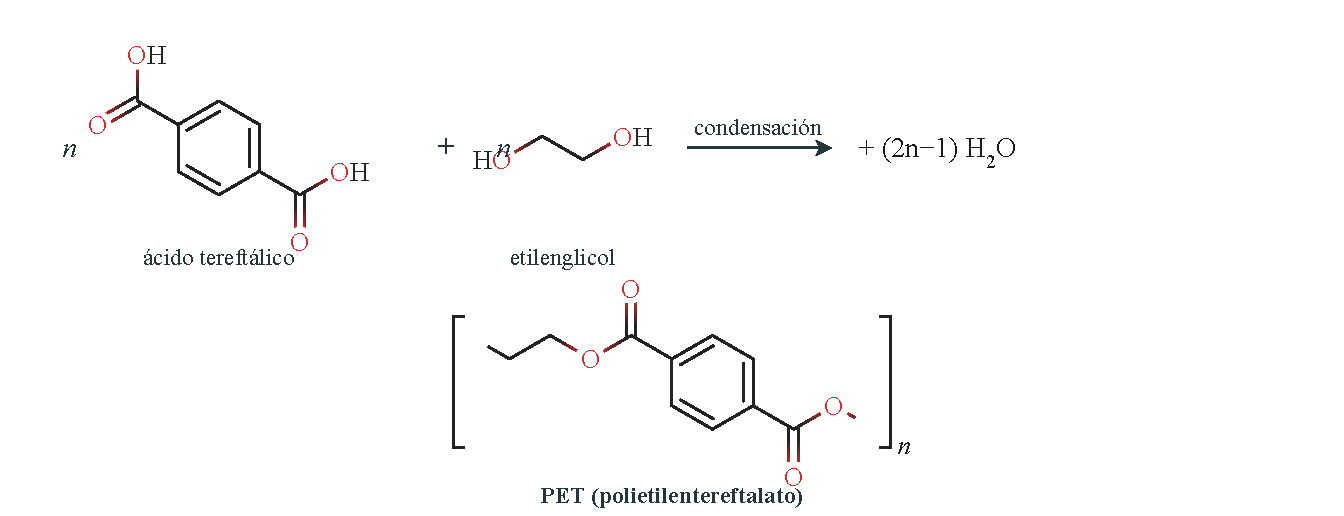
\includegraphics[width=0.95\linewidth]{FigurasSVG/UD10_Polimeros/pdf/UD10_06_formacion_PET.pdf}
            \caption{Formación del PET}
            \label{fig:formacion-pet}
        \end{figure}

        \textbf{Aplicaciones:}  fibra textil , envases de licores, medicamentos y alimentos, reparación de vasos sanguíneos…
        \item \negsubro{Poliamidas}. Son unos polímeros que contiene el grupo funcional amida en su cadena principal que se repite n veces.

        Se producen por sucesivas reacciones entre el grupo ácido y el amino. Para formar la función amida a los dos lados de la cadena se requiere que uno de los monómeros sea un diácido y el otro una diamina:

        La poliamida más conocida es el nailon 6,6  (conocido como seda artificial) formado por la copolimerización del ácido adípico  (ácido hexanodioico) y la 1,6-hexanodiamina:

        \begin{figure}[H]
            \centering
            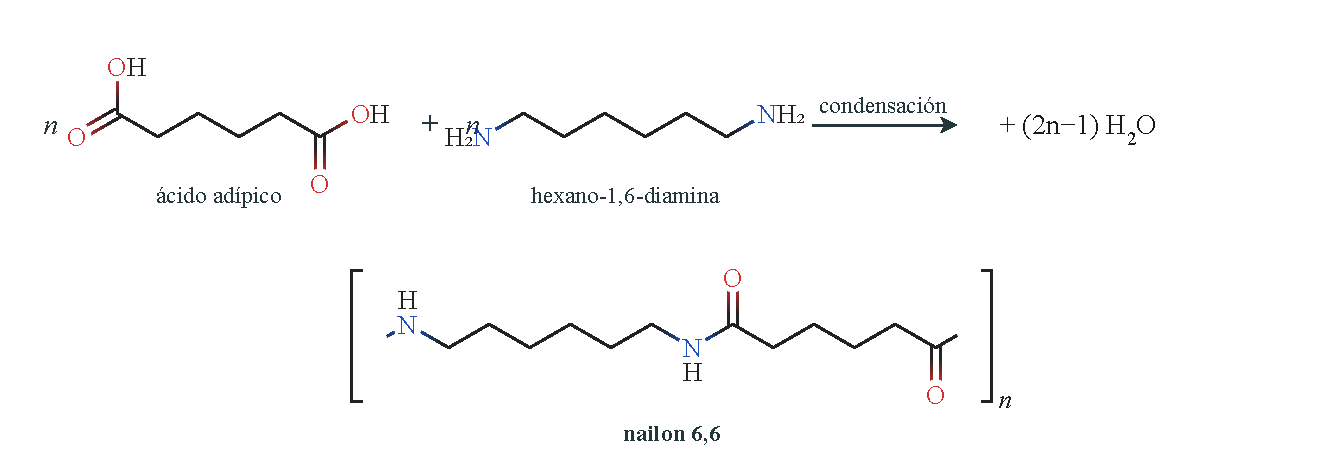
\includegraphics[width=0.95\linewidth]{FigurasSVG/UD10_Polimeros/pdf/UD10_07_formacion_nailon_66.pdf}
            \caption{Formación del nailon 6,6}
            \label{fig:formacion-nailon}
        \end{figure}

        Aplicaciones: Forma fibras muy resistentes por lo que se pueden utilizar para telas de paracaídas, sedales, medias, cepillos, cerdas, peines…


    \end{enumerate}





